%%%%%%%%%%%%%%%%%%%%%%%%%%%%%%%%%%%%%%%%%%%%%%%%%%%%%%%%%%%
%% Congratulations, you've made an excellent choice
%% of writing your Tampere University thesis using
%% the LaTeX system. This document attempts to be
%% as complete a template as possible to let you focus
%% on the most important part: the writing itself.
%% Thus the details regarding the visual appearance
%% and even structure have already been worked out
%% for you!
%%
%% I sincerely hope you will find this template useful
%% in completing your thesis project. I've tried to
%% add comments (followed by the % sign) to clarify
%% the structure and purpose of some of the commands.
%% Most of the magic happens in the file tauthesis.cls,
%% which you are more than welcome to take a look at.
%% Just refrain from editing it in the most crucial
%% versions of the thesis!
%%
%% I wish you and your thesis project the best of luck!
%% If this template causes you trouble along the way
%% or if you've any suggestions for improving it,
%% please be in contact through GitHub
%% (<URL HERE>)
%%
%% Yours,
%%
%% Ville Koljonen
%%
%% PS. This template or its associated class file don't
%% come with a warranty. The content is provided as is,
%% without even the implied promise of fitness to the
%% mentioned purpose. You, as the author of the thesis,
%% are responsible for the entire work, including the
%% provided material. No one else is liable to you for
%% any damage inflicted on you or your thesis, were it
%% caused by using this template or not.
%%%%%%%%%%%%%%%%%%%%%%%%%%%%%%%%%%%%%%%%%%%%%%%%%%%%%%%%%%%

%%%%% NOTICE %%%%%
%% Please read through the entire template
%% (files under ./tex) to find all instructions.
%% It is possible that the attached pdf files
%% do not include the latest information.
%%%%%%%%%%%%%%%%%%

%%%%% INSTRUCTIONS FOR COMPILING THE DOCUMENT %%%%%
%% Overleaf: just click Recompile.
%% Terminal:
%%  1. pdflatex main.tex
%%  2. makeindex -s main.ist -t main.glg -o main.gls main.glo
%%  3. biber main
%%  4. pdflatex main.tex
%%  5. pdflatex main.tex
%% Similar sequence of commands is also required
%% in LaTeX specific editors.
%%%%%%%%%%%%%%%%%%%%%%%%%%%%%%%%%%%%%%%%%%%%%%%%%%%

%%%%% METADATA %%%%%
%% Always keep the following metadata up to date!
%% This is important for your PDF file to comply
%% to accessibility standards.
%% (And yes, this information must remain here,
%% before \documentclass[...]{...}.)

% \Title and \Language are mandatory,
% others desirable
% The appropriate Finnish language code is 'fi',
% UK English is en-UK
\begin{filecontents*}[overwrite]{\jobname.xmpdata}
\Title{Palvelimien keskitetty hallinta Ansiblella}
\Author{Ville Nupponen}
\Language{fi}
\end{filecontents*}

\pdfminorversion=6

%%%%% PREAMBLE %%%%%

%%%%% Document class declaration.
% The possible optional arguments are
%   finnish - thesis in Finnish (default)
%   english - thesis in English
%   numeric - citations in numeric style (default)
%   authoryear - citations in author-year style
%   apa - citations in APA 7 (available only in English)
%   ieee - citations in IEEE style (available only in English)
%   draft - for faster non-final works, also skips images
%           (recommended, remove in final version)
%   programs - if you wish to display code snippets
% Example: \documentclass[english, authoryear]{tauthesis}
%          thesis in English with author-year citations
\documentclass[finnish, apa]{tauthesis}

% The glossaries package throws a warning:
% No language module detected for 'finnish'.
% You can safely ignore this. All other
% warnings should be taken care of!

%%%%% Your packages.
% Before adding packages, see if they can be found
% in tauthesis.cls already. If you're not sure that
% you need a certain package, don't include it in
% the document! This can dramatically reduce
% compilation time.

% Graphs
% \usepackage{pgfplots}
% \pgfplotsset{compat=1.15}

% Subfigures and wrapping text
% \usepackage{subcaption}

% Mathematics packages
\usepackage{amsmath, amssymb, amsthm}
%\usepackage{bm}

% Chemistry packages
% \usepackage{chemfig}
% \usepackage[version=4]{mhchem}

% Text hyperlinking
% \usepackage{hyperref}
% \hypersetup{hidelinks}

% (SI) unit handling
% \usepackage{siunitx}

%\sisetup{
%    detect-all,
%    math-sf=\mathrm,
%    exponent-product=\cdot,
%    output-decimal-marker={,} % for theses in FINNISH!
%}

\usepackage{listings}

%%%%% Your commands.

% Print verbatim LaTeX commands
\newcommand{\verbcommand}[1]{\texttt{\textbackslash #1}}

% Basic theorems in Finnish and in English.
% Remove [chapter] if you wish a simply
% running enumeration.
% \newtheorem{lause}{Lause}[chapter]
% \newtheorem{theorem}[lause]{Theorem}

% \newtheorem{apulause}[lause]{Apulause}
% \newtheorem{lemma}[lause]{Lemma}

% Use these versions for individually
% enumerated lemmas
% \newtheorem{apulause}{Apulause}[chapter]
% \newtheorem{lemma}{Lemma}[chapter]

% Definition style
% \theoremstyle{definition}
% \newtheorem{maaritelma}{Määritelmä}[chapter]
% \newtheorem{definition}[maaritelma]{Definition}
% examples in this style

%%%%% Glossary information.

% Use the following lines ONLY if you need more
% than one glossary. The first argument specifies
% a type label for the glossary and the second
% the displayed name.
% \newglossary*{symbs}{Symbols}
% \newglossary{label}{Displayed name}
% ...

\makeglossaries

% Use this line if using the default glossary.
% Otherwise comment out.
\loadglsentries[main]{tex/sanasto.tex}

% Use this line if using more than one glossary.
% Otherwise comment out.
% \loadglsentries[symbs]{tex/sanasto2.tex}

%%%%% Citation information.

% Commonly used bibliography modifications.
% Feel free to play around with them.

%\ExecuteBibliographyOptions{%
%sorting=none,
%maxbibnames=99,
%maxcitenames=2,
%giveninits=true,
%uniquename=init,
%sortcites,
%sortlocale=fin}

%\DefineBibliographyStrings{finnish}{%
%    in = {},
%    pages = {s.},
%    page = {s.}
%}
%\DefineBibliographyStrings{english}{%
%    in = {},
%    pages = {pp.},
%    page = {p.}
%}
%
%\DeclareNameAlias{sortname}{last-first}
%\DeclareNameAlias{author}{last-first}

%\DeclareFieldFormat[%
%    article,inbook,incollection,inproceedings,
%    patent,thesis,unpublished]{citetitle}{#1\isdot}
%\DeclareFieldFormat[%
%    article,inbook,incollection,inproceedings,
%    patent,thesis,unpublished]{title}{#1\isdot}
%\DeclareFieldFormat{pagetotal}{#1 \bibstring{page}}

%\AtBeginBibliography{\renewcommand*{\makelabel}[1]{#1\hss}}

%\DefineBibliographyExtras{english}{\let\finalandcomma=\empty}

\addbibresource{tex/references.bib}

\begin{document}

%%%%% FRONT MATTER %%%%%

\frontmatter

%%%%% Thesis information and title page.

% The titles of the work. If there is no subtitle,
% leave the arguments empty. Pass the title in
% the primary language as the first argument
% and its translation to the secondary language
% as the second.
\title{Palvelimien keskitetty hallinta Ansiblella}{Centralized management of servers with Ansible}
\subtitle{Ansiblen perusteet ja yleisimpiä aloittelijan virheitä}{Ansible basics and common beginner mistakes}

% The author name.
\author{Ville Nupponen}

% The examiner information.
% If your work has multiple examiners, replace with
% \examiner[<label>]{<name> \\ <name>}
% where <label> is an appropriate (plural) label,
% e.g. Examiners or Tarkastajat, and <name>s are
% replaced by the examiner names, each on their
% separate line.
\examiner[Tarkastajat]{Petri Kannisto}

% The finishing date of the thesis (YYYY-MM-DD).
\finishdate{2022}{04}{24}

% The type of the thesis (e.g. Kandidaatintyö
% or Master of Science Thesis) in the primary
% and the secondary languages of the thesis.
\thesistype{Kandidaatintyö}{Bachelor's thesis}

% The faculty and degree programme names in
% the primary and the secondary languages of
% the thesis.
\facultyname{Informaatioteknologian ja viestinnän tiedekunta}{Faculty of Information Technology and Communication Sciences}
\programmename{Tietotekniikka}{Computing Sciences}

% The keywords to the thesis in the primary and
% the secondary languages of the thesis
\keywords%
    {IaC, Infrastructure as Code, Ansible, Tietoturvahajut, Huonot käytännöt, Ansible-lint}

\maketitle

%%%%% Abstracts and preface.

% Write the abstract(s) and the preface
% into a separate file for the sake of clarity.
% Pass the appropriate file name as the first
% argument to these commands. Put the \abstract
% in the primary language first and the
% \otherabstract in the secondary language second.
% Those who do not speak Finnish only need the
% first abstract. The second argument of
% the \preface command takes the place where
% the thesis was signed in.
\abstract{tex/tiivistelma.tex}
% \otherabstract{tex/abstract.tex}
% \preface{tex/alkusanat.tex}{Tampereella}

%%%%% Table of contents.

\tableofcontents

%%%%% Lists of figures, tables, listings and terms.

% Print the lists of figures and/or tables.
% Uncomment either of these commands as required.
% Both are optional, but if there are many important
% figures/tables, listing them may be a good idea.

% \listoffigures
% \listoftables
% \lstlistoflistings

% Misc stuff related to how the glossary is displayed.
% You can especially tweak the lengths to suit you!
\glsaddall
\setglossarystyle{taulong}
\setlength{\glsnamewidth}{0.25\textwidth}
\setlength{\glsdescwidth}{0.75\textwidth}
\renewcommand*{\glsgroupskip}{}

% Print the default glossary of abbreviations,
% if necessary. Otherwise comment out.
% The appropriate Finnish variant is 'Lyhenteet'
\printglossary[title={Lyhenteet ja merkinnät}]

% Print more than one glossary with these lines.
% Otherwise comment out.
% \printglossary[type=symbs]
% \printglossary[type=label]
% ...

%%%%% MAIN MATTER %%%%%

\mainmatter

% Write each of the chapters of the thesis
% into a separate file for the sake of clarity.
% They can be \input as shown below. Give both
% the chapters and their files as descriptive
% names as possible.
\chapter{JOHDANTO}
\label{ch:johdanto}
Tämä mallipohja liittyy Tampereen yliopiston tekniikan alan opinnäytteiden kirjoitusohjeisiin \parencite{kirjoitusohje2018}. Opinnäyte koostuu tyypillisesti seuraavista osista:

\begin{enumerate}
    \item[] Nimiölehti
    \item[] Tiivistelmä suomeksi ja englanniksi
    \item[] Alkusanat
    \item[] Sisällysluettelo
    \item[] (Kuva- ja taulukkoluettelot)
    \item[] Lyhenteet ja merkinnät
    \item Johdanto
    \item Teoreettinen tausta, lähtökohdat tai ongelman asettelu
    \item Tutkimusmenetelmät ja aineisto
    \item Tulokset ja niiden tarkastelu (mahdollisesti eri luvuissa)
    \item Yhteenveto ja/tai päätelmät
    \item[] Lähdeluettelo
    \item[] (Liitteet)
\end{enumerate}

Jokainen yllämainituista osista kirjoitetaan omaksi luvukseen (\verbcommand{chapter}) tai asianmukaisella komennolla (esim. \verbcommand{abstract}). Lue pohja ja sen kommentit huolella läpi. Osioiden 1--5 nimet ovat tässä ainoastaan esimerkkejä. Käytä työssäsi paremmin sisältöä kuvaavia nimiä. Nimiölehti luodaan täyttämällä asianmukaiset tiedot komentoihin pohjan alkupuolella. Sisällysluetteloon kootaan kaikki sitä seuraavat otsikot, erityisesti numeroidut. Aina siihen ei laiteta osia ennen sisällysluetteloa.

Johdannossa herätetään lukijan mielenkiinto, perehdytetään hänet tutkimuksen aihepiiriin ja jäsennetään tutkimus. Seuraavaksi esitellään opinnäytetyön taustatiedot, jotka ovat välttämättömiä työn ongelman ymmärtämiselle. Toisinaan tässä kuvataan myös käytetyt menetelmät ja aineisto, eli miten tutkimus on toteutettu.

Sen jälkeen esitellään työssä saavutetut tulokset, niiden merkitys, virhelähteet, poikkeamat oletetuista tuloksista ja tulosten luotettavuus. Yhteenveto on työn tärkein osio. Siinä ei enää toisteta yksityiskohtaisen tarkkoja tuloksia, vaan päätulokset kootaan yhteen ja pohditaan niiden merkitystä. Lähdeluettelo antaa kuvan työn teoreettisesta ja empiirisestä pohjasta sekä toimii kirjallisuusluettelona. Siinä esitetään kaikki tarvittavat tiedot kunkin julkaisun löytämiseksi.

Tämän pohjan luvussa \ref{ch:esitystyyli} käsitellään kuviin, taulukoihin ja matemaattisiin merkintöihin liittyvät esitystyylin perussäännöt. Luvuissa \ref{ch:viittaustekniikat} ja \ref{ch:yhteenveto} esitellään viittaustekniikat ja lyhyt yhteenveto. Jokaisessa kohdassa annetaan lisäksi vinkkejä joidenkin yksityiskohtien ratkaisemiseen \LaTeX{}illa.

\chapter{ANSIBLE PERUSTEET}
\label{ch:perusteet}
Ansible on yksi monista eri vaihtoehdoista toteuttaa infrastruktuuri koodina.
Tässä luvussa esitellään lyhyesti, mitä infrastruktuuri koodina on ja
mitä eri vaihtoehtoja on. Tämän lisäksi käydään läpi Ansiblen perusteita,
joiden tietäminen on välttämätöntä myöhempien lukujen kannalta.

\section{Infrastruktuuri koodina}

Infratruktuuri koodina on nimensä mukaisesti sitä, että infrastruktuuri
muodostetaan koodin pohjalta. Lähtökohtaisesti ympäristö on tällöin
luotu automaattisesti ja määritellyllä tavalla, ja se on mahdollista
toteuttaa uudelleen samanlaisena. Infrastruktuurin toteuttaminen koodin
avulla mahdollistaa koko infrastruktuurin dokumennoin toteutuksen ohessa
eikä jätä ympäristöön liittyviä asioita tekijän muistin varaan.
\parencite{KiefMorris2020IaC2}

Tunnettuja IaC-ratkaisuja ovat muun muassa Ansible, Puppet, Chef, SaltStack
ja Terraform. Idea eri ratkaisuissa on pääpiirteittä sama. Suurimpia eroja
tuovat kieli, jolla ratkaisu on toteutettu sekä ajamisessa käytettävä
metodi. Osa ratkaisuista, kuten Chref ja Puppet, suosivat veto-metodia,
kun puolestaan Ansible ja Terraform työntö-metodia. Veto-metodissa
käyttäjä suorittaa ohjelman palvelimella, jolle haluaa tehdä muutoksia.
Tällöin ohjelma hakee tarvittavat määritykset keskitetyltä hallintapalvelimelta.
Työntö-metodissa puolestaan ohjelma ottaa yhteyden halutulle palvelimille,
toteuttaakseen käyttäjän määrittämät toiminnot. \parencite{RitiPierluigi2021IaC}

\section{Ansiblen asennus ja käyttö}

Versiosta 2.10 alkaen Ansible on jakautunut kahteen eri pakettiin:
ansibleen ja ansible-coreen. Varsinainen Ansiblen ydin löytyy
ansible-core-paketista. Ansible paketti puolestaan sisältää yhteisön
tarjoaman valmiin kattauksen moduuleja, joita voidaan käyttää eri
tehtävissä. \parencite{AnsibleDocs}

Ansible tarvitsee toimiakseen Pythonin, joten käyttöjärjestelmästä
löytyy todennäköisesti myös Pythonin pakettemanageri eli Pip, jolla
Ansiblen asennus onnistuu vaivattomasti:

\begin{lstlisting}[
    basicstyle=\small,
    label={lst:install-ansible},
    language=bash
]
    $ pip3 install ansible
\end{lstlisting}

Tämän jälkeen voidaan toiminnallisuus testata esimerkiksi:

\begin{lstlisting}[
    basicstyle=\small,
    label={lst:ansible-ping},
    language=bash
]
    $ ansible localhost -m ping
\end{lstlisting}

\subsection{Inventaario}

Ansiblella hallittavat palvelimet luetteloidaan inventaariossa.
Yksinkertaisimmillaan inventaario sisältää listan palvelimien nimistä
esimerkin \ref{lst:ansible-inventory} mukaisesti.
\parencite{JamesFreeman2020PA2}

\begin{lstlisting}[
    basicstyle=\small,
    label={lst:ansible-inventory},
]
    mail.example.com

    [webservers]
    foo.example.com
    bar.example.com

    [dbservers]
    one.example.com
    two.example.com
    three.example.com
\end{lstlisting}

Inventaariot voivat myös olla dynaamisia \parencite{JamesFreeman2020PA2}.
Tällöin lista palvelimista voidaan hakea esimerkiksi palveluntarjoajan
ohjelmointirajapinnasta. \parencite{AnsibleDocs}.

\subsection{Playbookit ja tehtävät}

Ansiblessa suoritaan yksittäisiä pieniä tehtäviä, joita peräkkäin ajamalla
saadaan toteutettua kokonaisuuksia. Tehtävät käyttävät jotain asennettua
moduulia. \parencite{JamesFreeman2020PA2} Esimerkissä \ref{lst:ansible-apt-figlet}
käytetään apt-moduulia, jolla saadaan asennettua määritelty paketti. Esimerkin
mukaisesti tehtäville annetaan kuvaava nimi, joka tulee näkymään myöhemmin
ulostulossa kun, tehtäviä ajetaan.

\lstinputlisting[
    basicstyle=\small,
    caption={Figlet-ohjelman asentaminen Ansiblen apt-moduulilla},
    label={lst:ansible-apt-figlet},
]{code/install-figlet.yaml}

Playbookit puolestaan määrittelevät rooleista ja tehtävistä muodostuvia
kokonaisuuksia. \parencite{JamesFreeman2020PA2}

\lstinputlisting[
    basicstyle=\small,
    caption={Esimerkki playbookista},
    label={lst:ansible-playbook},
]{code/playbook-example.yaml}

Esimerkissä \ref{lst:ansible-playbook} on määritelty hcloud-ryhmälle, joka
saadaan haettua inventaariosta, ajettavaksi ensimmäisenä yksittäinen tehtävä
ja tämän jälkeen kaksi roolia.

Playbook saadaan ajettua ansible-playbook -komennolla:

\begin{lstlisting}[
    basicstyle=\small,
    label={lst:run-ansible-playbook},
    language=bash
]
    $ ansible-playbook -i inventory.ini playbook.yml
\end{lstlisting}

\subsection{Roolit, sapluunat ja käsittelijät}

Yksittäisten tehtävien kirjoittamisen sisään on mahdollista tehdä rooleja,
jotka sisältävän useita tehtäviä ja muita niiden tarvitsemia asioita, kuten
sapluunoita (template) tai käsittelöitä (handlers). Samaa roolia voidaan
käyttää myös useissa eri playbookeissa, jolloin rooleilla saadaan muodostettua
pieniä kokonaisuuksia, joita yhdistelemällä saadaan muodostettua koko
kokonaisuus. \parencite{JamesFreeman2020PA2} Roolin kansiorakenne on esimerkin
\ref{lst:ansible-role-structure} mukainen \parencite{AnsibleDocs}.

\begin{lstlisting}[
    basicstyle=\small,
    label={lst:ansible-role-structure},
]
    roles/
        example-role/
            tasks/
            handlers/
            library/
            files/
            templates/
            vars/
            defaults/
            meta/
\end{lstlisting}

Yksinkertaisimmillaan rooli sisältää vain tasks-kansion, jossa on määritelty
main.yml-tiedosto, joka sisältää kaikki roolin ajettavat tehtävät. Rooli
voi siis käytännössä olla vain yksi tehtävä, kuten aiemmin esitelty esimerkki
yksittäisestä tehtävästä \ref{lst:ansible-apt-figlet}.

Roolit voivat sisältää myös muita hyödyllisiä työkaluja, kuten sapluunoita tai
käsittelijöitä. Sapluunoiden avulla voidaan rakentaa esimerkiksi ohjelman
asetustiedostolle pohja, johon täytetään tiedot palvelinkohtaisesti. Sapluuna
muodostetaan jinja2-kieltä käyttämällä. \parencite{JamesFreeman2020PA2}

\lstinputlisting[
    basicstyle=\small,
    caption={Esimerkki käyttäjän ssh-avaimien listaamisesta},
    label={lst:template-example},
]{code/template-example.j2}

Jinja2-kieli tukee datan yksinkertaista käsittelyä, kuten esimerkin
\ref{lst:template-example} mukaisesti listojen läpi käyntiä. Sapluunoja
käytetään template-moduulin avulla, josta on esimerkki käsittelijä-esimerkin
yhteydessä \ref{lst:handler-task-example}. \parencite{AnsibleDocs}

Ohjelmien asennus voi vaatia useita pieniä tehtäviä, jotta ohjelma toimii
oikein. Tällöin ohjelman käynnistämistä ei voida välttämättä toteuttaa ennen
kuin kaikki tehtävät on suoritettu. Tällöin on mahdollista merkittävä tehtäville
käsittelijä. Käsittelijä ajetaan vasta, kun kaikki tehtävät on suoritettu.
Yleinen käyttö käsittelijöille  on nimenomaan asetustiedostojen yhteydessä.
Käsittelijä ajetaan vain jos tehtävä, johon se on liitetty, tekee muutoksia.
Tällöin voidaan esimerkiksi käynnistää ohjelma uusiksi mikäli asetustiedostossa
on muutoksia ja ohjelma tarvitsee uudelleenkäynnistyksen ladatakseen uudet
muutokset. \parencite{JamesFreeman2020PA2}

Käsittelijä laitetaan handlers-kansioon main.yml-tiedostoon esimerkin
\ref{lst:handler-example} mukaisesti.

\lstinputlisting[
    basicstyle=\small,
    caption={Esimerkki käsittelijän toteuttamisesta},
    label={lst:handler-example},
]{code/handler-example.yaml}

Määriteltyjä käsittelijöitä voidaan käyttää tehtävän yhteydessä notify-avainsanan
avulla, kuten esimerkissä \ref{lst:handler-task-example} on näytetty.

\lstinputlisting[
    basicstyle=\small,
    caption={Esimerkki käsittelijän toteuttamisesta},
    label={lst:handler-task-example},
]{code/handler-task-example.yaml}

\subsection{Muuttujat ja holvi}

Ansiblessa tietoa säilytään muuttujissa. Muuttujia on mahdollista määrittää monella
eri tavalla. Muuttujat on voitu määritellä esimerkiksi roolissa, inventorissa
tai playbookissa ja ne voivat kohdistua tiettyyn palvelimeen tai palvelimien
muodostomaan ryhmään. \parencite{JamesFreeman2020PA2}

Muuttujiin saatetaan kuitenkin haluta määritellä salasanoja tai muida arkaluontoisia
tietoja. Jotta arkaluontoiset tiedot saadaan salattua, voidaan käyttään Ansiblen
tarjoamaa holvia. \parencite{JamesFreeman2020PA2}

\begin{lstlisting}[
    basicstyle=\small,
    label={lst:ansible-vault},
    language=bash
]
    $ pwgen -s 77 1 | tr -d '\n' | ansible-vault encrypt_string \
        --vault-password-file ansible-vault.secret \
        --encrypt-vault-id default
    Reading plaintext input from stdin. (ctrl-d to end input, twice if
    your content does not already have a newline)

    !vault |
              $ANSIBLE_VAULT;1.1;AES256
              3538646364656536356461313931323831356638643831396135623836
              3563303363643561613032376639646534303366633533333539626535
              3938393536360a63376136303037303037613936316532656561366462
              3335363136313533616331646132633433346330303865363332636135
              346436313331633664396532620a323439626639376666333634333536
              3461313664623036613130363931616231303631383130396261386634
              3134393439326538386665633436306562663330366535666365633232
              3039646361333636333330323035313334396134363232636461333033
              3566373664313361356135616330363838653832613536396639383339
              6164366463343736623635633035393962303933373662666237636633
    Encryption successful

\end{lstlisting}

Esimerkissä \ref{lst:ansible-vault} generoidaan satunnainen 77-merkkinen salasana,
joka sen jälkeen välitetään ansible-vault -komennolle, joka salaa generoidun
salasanan ansible-vault.secret -tiedoston avulla. Tämän jälkeen salattua tietoa
voidaan käyttää muuttujien sisältönä esimerkin \ref{lst:var-example} mukaisesti.

\lstinputlisting[
    basicstyle=\small,
    caption={Muuttujien määrittely},
    label={lst:var-example},
]{code/var-example.yaml}

Kunhan vain Ansible pystyy saamaan tiedoston, jonka avulla salaus toteutettiin,
pystyy Ansible purkamaan salaisuuden ajon yhteydessä. Nyt on vain huolehdittava
salaamisessa käytettävän tiedoston välittämisestä kaikille sitä tarvitseville ja
kaikki muut salaisuudet voivat olla versionhallinnassa.


\chapter{HAVAITTUJA VIRHEITÄ}
\label{ch:virheet}
TODO: Virheet

\chapter{VIRHEIDEN AUTOMAATTINEN TUNNISTAMINEN}
\label{ch:virheiden-havaitseminen}
Tutkimuksissa \parencite{RahmanAkond2019TSSS} ja \parencite{RahmanAkond2021SSiA} käytettiin
tutkimuksia varten tehtyjä työkaluja, jotka oli empiirisesti validoitu toimiviksi.
Kyseiset työkalut eivät yleisesti ole tiedossa tai käytettävissä. Tässä luvussa on
kuitenkin esitelty yksi työkalu, Ansible Lint, joka edes auttaa havaitsemaan vastaavia
virheitä ja johon on mahdollista rakentaa itse lisätarkistuksia \parencite{SestoVincent2020ATaV}.

\section{Ansible Lint}

Ansible Lint on työkalu, joka on suunniteltu tarkistamaan noudatetaanko parhaita
käytäntöjä ja sen myötä edesauttamaan käytäntöjen parantamista \parencite{GithubAnsibleLint}.
Työkalua ei ole nimenomaan suunniteltu huomaamaan turvallisuuspuutteita, mutta parhaat
käytännöt sisältävät myös asioita, jotka ovat turvallisuuden kannalta oleellisia.

\subsection{Manuaalinen ajaminen}

Ansible vaatii ajamiseen tarkoitetulla palvelimella Python 3.8:n \parencite{AnsibleDocs}.
Tämän myötä koneelle on todennäköisesti asennettu myös pip. Työkalun asentaminen
onnistuukin tällöin helposti pipin avulla \parencite{AnsibleLintReadTheDocs}:

\begin{lstlisting}[
    basicstyle=\small,
    label={lst:install-ansible-lint},
    language=bash
]
    $ pip3 install ansible-lint
\end{lstlisting}

Työkalu ei tarvitse lisämäärityksiä vaan voi tunnistaa automaattisesti tarvittavat
tiedostot Ansible-projektista \parencite{AnsibleLintReadTheDocs}:

\begin{lstlisting}[
    basicstyle=\small,
    label={lst:run-ansible-lint},
    language=bash
]
    $ ansible-lint
\end{lstlisting}

Komennon antama ulostulo voi näyttää esimerkin \ref{lst:Ansible Lint-simple-example} mukaiselta.

\begin{lstlisting}[
    basicstyle=\small,
    label={lst:ansible-lint-simple-example},
    breaklines=true,
]
    no-handler: Tasks that run when changed should likely be handlers
    hcloud_roles/hcloud_server/tasks/main.yml:119 Task/Handler: Discord notification

    risky-file-permissions: File permissions unset or incorrect
    roles/address_checker/tasks/main.yml:13 Task/Handler: DB volume directory
\end{lstlisting}

Kattavampi ulostulo on esitelty liitteessä \ref{lst:ansible-lint-example}. Liitteestä
nähdään kuinka kehittäjältä jää helposti useita yksinkertaisia ongelmia huomaamatta ja
saman ongelman toistuvan useasti.

\subsection{Automaattinen ajaminen Gitlab CI:n avulla}

Gitlabia tietovarastona (repository) käyttävät ohjelmistoprojektit voivat käyttää
jatkuvan integraation ja kehittämisen suorittamiseen Gitlab CI/CD:ta, joka mahdollistaa
erilaisten tehtävien suorittamisen automaattisesti koodivarantoon tehtyjen muutoksien
perusteella. Gitlab CI/CD perustuu avoimeen lähdekoodiin ja sen ilmainen versio on ollut
jo aikoinaan parhaimpia ja kattavampia. \parencite{alma9911268330505973}

Yleisesti tunnettuja vaihtoehtoisia ratkaisuja ovat muun muassa Github Actions,
Travis CI, CircleCI ja Jenkins. Tässä työssä kuitenkin esitellään toteutus vain
Gitlab CI/CD:llä, sillä muilla toteuttaminen tapahtuu vastaavasti.

Gitlab CI:ssa tarvittavat määritykset laitetaan `.gitlab-ci.yml`-tiedostoon
\parencite{GitlabCICDDocs}. Esimerkissä \ref{lst:gitlab-ci-ansible-lint} esitelty
yksinkertainen vaihtoehto, jolla saadaan ajettua `ansible-lint` automaattisesti
jokaisen muutoksen myötä.

\lstinputlisting[
    basicstyle=\small,
    caption={Esimerkki yksinkertaisesti Gitlab CI määrityksestä Ansible Lint:n ajamiseen automaattisesti},
    label={lst:gitlab-ci-ansible-lint},
]{code/gitlab-ci-ansible-lint.yaml}

Ylläoleva esimerkki on yksinkertainen eikä sisällä esimerkiksi välimuistin
määrittämistä, jottei työkaluja tarvitse jokaisella suorituskerralla asentaa
uusiksi. Lisäksi työkalun ajaminen joka ei kerta ei välttämättä ole suositeltava
ratkaisu mikäli muutokset eivät kohdistuneen mihinkään, joka vaikuttaisi
lopputulokseen.

\subsection{Tulosten näyttäminen Gitlabissa}

Gitlab CI vertailee koodinlaaturaportteja eri haarojen välillä ja näyttää
tulokset Gitlabin käyttöliittymän kautta \parencite{GitlabCICDDocs}. Kuvassa
\ref{fig:gitlab-code-quality-improved} on näytetty esimerkki siitä, kun
koodin laatu paranee muutosten myötä.

\begin{figure}[h!]
    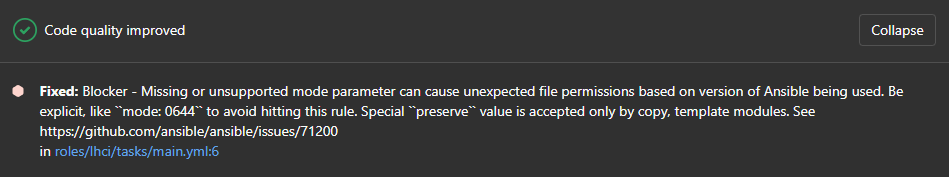
\includegraphics[width=\textwidth]{figures/gitlab-code-quality-improved}
    \caption{Kuvankaappaus Gitlabin Merge Requestin yleiskatsauksesta}
    \label{fig:gitlab-code-quality-improved}
\end{figure}

On hyvä huomioida, että kohdehaarassa tulee olla muodostettu vastaava raportti
vähintään kerran, jotta vertailua voidaan suorittaa. Muodostetut raportin on
mahdollista ladata Gitlabin käyttöliittymän kautta.\parencite{GitlabCICDDocs}


\chapter{YHTEENVETO}
\label{ch:yhteenveto}
Ohjeilla pyritään mahdollisimman selkeään ja täsmälliseen tekstiin, joka on tärkeää kaikissa kirjallisissa raporteissa. Tämän dokumenttipohjan ja vastaavan Word-pohjan avulla töillä on yhtenäinen ja selkeä ulkoasu.

Jokaisella kirjoituksella ja esityksellä pitää olla yhteenveto. Tätä asiaa korostetaan lisäämällä sellainen tähänkin pohjaan, vaikkakin lyhyenä ja hieman keinotekoisesti. Tiivis yhteenvetotaulukko voi auttaa kertaamaan tärkeimmät kohdat.

Lopuksi vielä mainintoja tästä pohjasta. Valmiin dokumentin tuottamiseksi se on käännettävä pdf\LaTeX{}-ohjelmalla. Tämä vaihtoehto on varsin helposti löydettävissä valmiissa \LaTeX{}-editoreissa, ja komentoriviä käyttäessä riittää kirjoittaa komennoksi \texttt{pdflatex}. Viitteiden ja lähdeluettelon luomiseksi käytetään biber-nimistä ohjelmaa, joka löytyy samaan tapaan. Lyhenne- ja symboliluettelon latomiseksi täytyy ajaa makeindex-niminen ohjelma. Jos vaikuttaa siltä, että sisällysluettelo tai ristiinviittaukset (\verbcommand{ref}) eivät näy oikein, kokeile ajaa pdf\LaTeX{} uudestaan. Jos lopultakin kääntäjä antaa virheraportteja, varmista ensin, että \TeX{}-asennuksesi on ajan tasalla.

Pohja on kirjoitettu Overleaf-ympäristössä, ja kirjoittaja suositteleekin lämpimästi sen version 2 käyttöä opinnäytteiden kirjoittamisessa. Helpoin keino päästä käsiksi dokumenttipohjaan on pyytää kopiointilinkkiä tähän projektiin työn ohjaajalta tai pohjan ylläpitäjältä. Overleafin käyttö vaatii kuitenkin käyttäjätilin ja verkkoyhteyden.

Toivon mukaan ajantasainen versio löytyy myös yliopiston intrasta. Pohja on testattu ja todettu toimivaksi Windows-käyttöjärjestelmän Mik\TeX-ympäristössä ja Unix-järjestelmien täydessä \TeX{} Live -ympäristössä. Näistä ensimmäinen asentaa automaattisesti mahdollisesti puuttuvia paketteja, mutta jälkimmäisen kanssa voi joutua etsimään ja asentamaan itse kokonaisia paketteja tai niiden päivitysversioita.

%%%%% Bibliography/references.

% Print the bibliography according to the
% information in ./tex/references.bib and
% the in-line citations used in the body of
% the thesis.
% \emergencystretch=2em
\printbibliography[heading=bibintoc]

%%%%% Appendices.

% Use only if it clarifies the structure of
% the document. Remember to introduce each
% appendix and its content.

\begin{appendices}

\chapter{Ansible-lint komennon ulostulo}
\label{ch:liite}
Tämä teksti toimii esimerkkinä liitteiden muodostamiseen tässä dokumenttipohjassa. Vähän pidempi saa siitä kokonaisen kappaleen näköisen.


\end{appendices}

\end{document}